
\begin{figure}[t]
	\centering
		\begin{minipage}{0.225\textwidth}
			\centering
			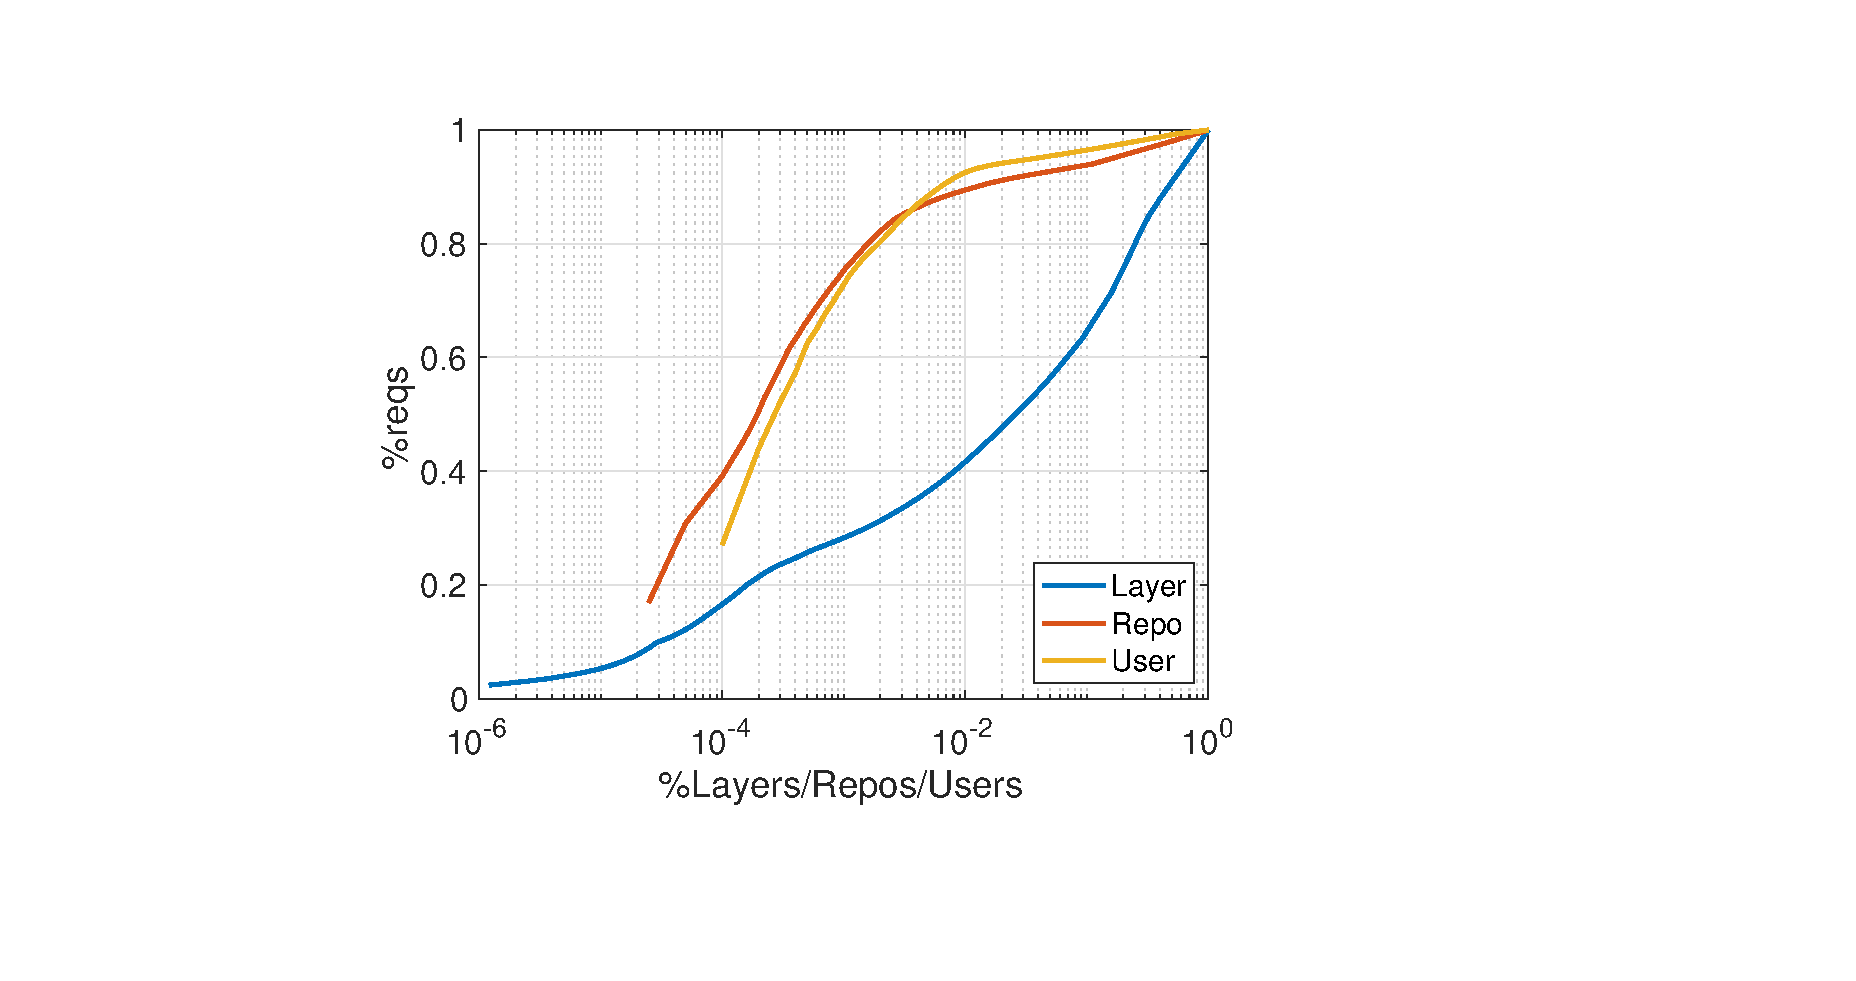
\includegraphics[width=1\textwidth]{graphs/skewness_cdf.eps}
			\caption{Popularity of layers, repos, and users.}
			\label{fig:sknewss}
		\end{minipage}
	\begin{minipage}{0.225\textwidth}
		\centering
		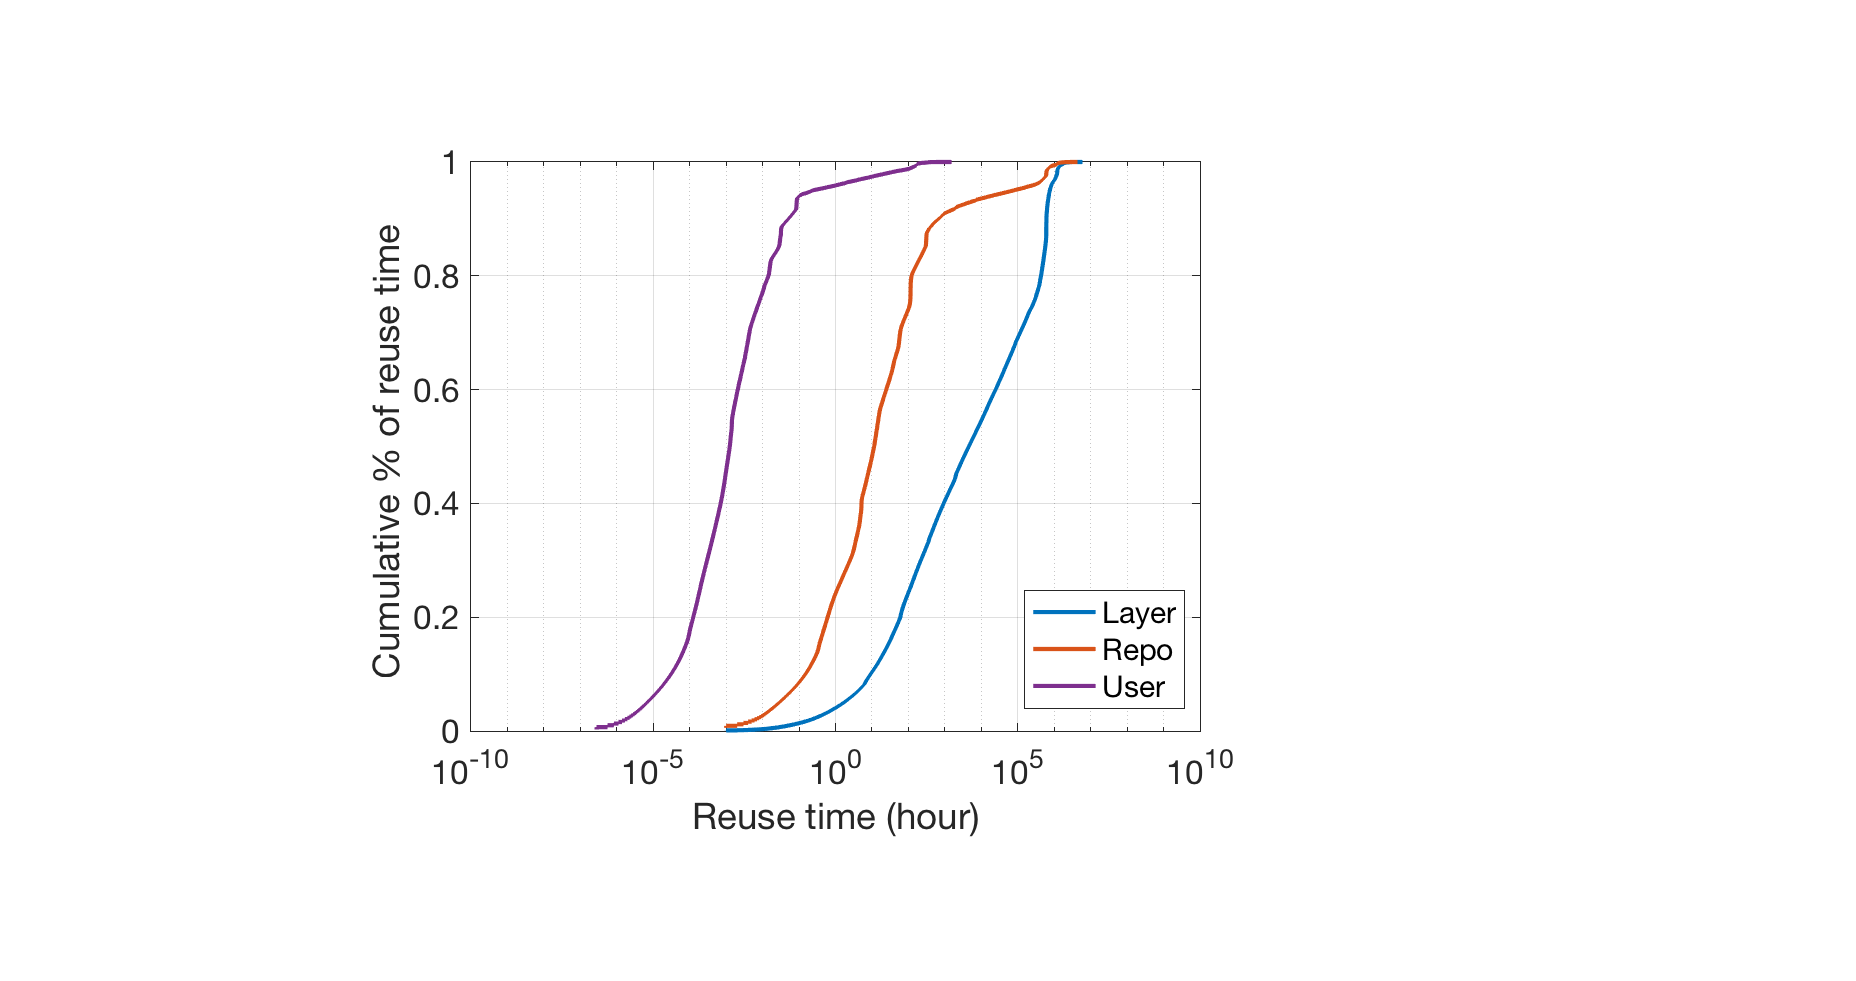
\includegraphics[width=1\textwidth]{graphs/reuse_time.eps}
		\caption{CDF of reuse time for layers, repos, and users.}
		\vspace{-3pt}
		\label{fig:reusetime}
	\end{minipage}
\end{figure}

\paragraph{Understanding layer access patterns.}
We analyzed the Dallas(\texttt{dal}) registry workload collected from IBM Container Registry over the course of 75 days~\cite{dockerworkload}. 
Figure~\ref{fig:sknewss} shows the registry accesses to layers and repositories, as well as users accesses to the layers and manifests.
% \arb{layers??}\NZ{addressed}. 
Layer accesses are heavily skewed. For example, $25$\% of popular layers account for $80$\% of all requests. 
For repository accesses and accesses by users, the skew is more significant than it is for layers. %10\% most frequently accessed repositories account for 94\% of all requests
$94$\% of all requests accessed only $10$\% of the (popular) repositories. Similarly, only $9$\% of (most active) users issued $97$\% of all requests. 
This means that only a few extremely active users create their repositories in the \texttt{dal} registry and issue the majority of requests to the registry.

Figure~\ref{fig:reusetime} shows the reuse time of layers and repositories and users.
Layer reuse time is the duration between two consecutive requests to the same layer or repository. Similarly,
reuse time by user is duration between two consecutive same-user requests.
The layer reuse time is long.
The median reuse time of a layer is $1.3$ hours. $80$\% of repositories experience the highest request frequency, with a reuse time of $2$ minutes. 
$90$\% of users remain active for at least $0.06$ seconds, thus most layers are not requested within a short time period.
%So for a registry, most of its stored layers are not accessed frequently given a very short time period while
%users can maintain active for a longer time. 
%This is because users can access multiple layers and manifests.
%   Thus, most of the layers stored in the
%   registry are not frequently requested over very short
%   time periods.
%, while users remain active for a longer time.
%This is because users can request different layers or manifests.

To quantify the efficacy of traditional LRU and push-pull prefetching,
we implemented an LRU algorithm and push-pull prefetching~\cite{dockerworkload} 
and replayed 
IBM registry workload \texttt{dal} with different cache size as shown in 
Figure~\ref{fig:lru_prefetching_hits}.
The hit ratio for LRU was found to be lower than $60$\% across different sizes.
This is because layer accesses do not follow LRU temporal trend:
recently pulled layer will not be pulled again by the same user.
Although push-pull prefetching slightly improved the hit ratio compared to LRU,
the maximum hit ratio is still low and stays stable around $80$\%.
This is because push-pull prefetching predicts the future accesses based on  
pushed layers.
However, based on our above trace analysis,
only half of the \texttt{pull} layer
requests have a preceding \texttt{push} layer request within the trace
%collecting duration
collection period of 75 days. This means that, after a user pushes a layer
to the registry, it takes a few days, weeks, or even months for a user to make
a \texttt{pull} request. 
%Second, we found in the traces only half of the pull layer requests have a preceding 
%push layer request and push-pull prefetching ignored the layers that were pushed 
%before data collection.

%Anwar et
%al. have proposed a prefetching method~\cite{dockerworkload} based on the
%\texttt{push}-\texttt{pull} relationship: whenever there is a \texttt{PUSH} layer
%request directly followed by a \texttt{GET} manifest request, with a high probability these will be followed by a \texttt{GET}
%layer request.


%\arb{say something whether this is good or bad... or is very low and show that LRU is not an effective mechanism for managing the proposed caches}\NZ{addressed}

